O método da Divisão áurea é outro método de localização de mínimos de funções escalares. Foi criado como uma avanço para o método de Fibonacci e se baseia na razão áurea. Por definição, para dividir o segmento de reta da figura \ref{fig:abc} na razão áurea, é necessário que

\begin{equation*}
\dfrac{\overline{AC}}{\overline{AB}} = \dfrac{\overline{AB}}{\overline{BC}}
\end{equation*}

\begin{figure}[h]
	\begin{center}
		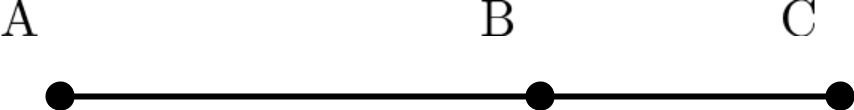
\includegraphics[width=8cm]{../aurea/dots_a_b_c.png}   
		\caption{Segmento de reta $ \overline{ABC} $}
		\label{fig:abc}
	\end{center}
\end{figure}

Dessa relação, podemos deduzir que $ \overline{AB} = 0.618\overline{AC} $. Assim, o segmento de reta fica dividido segundo a razão áurea, como mostra a figura \ref{fig:aurea_abc}.

\begin{figure}[h]
	\begin{center}
		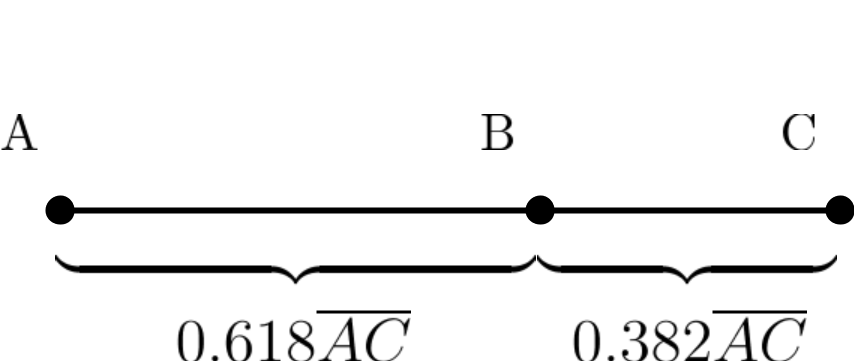
\includegraphics[width=8cm]{../aurea/dots_a_b_c_aurea.png}   
		\caption{Divisão áurea do segmento de reta}
		\label{fig:aurea_abc}
	\end{center}
\end{figure}

A sequência de Fibonacci, base para a construção do método de Fibonacci, tem uma semelhança com a razão áurea: A divisão entre dois números consecutivos dessa sequência converge para a razão áurea. Ou seja, o método da divisão áurea tenta aprimorar o método de Fibonacci porque desde a primeira iteração, já faz a divisão do intervalo para o melhor possível.

\begin{figure}[h]
	\begin{center}
		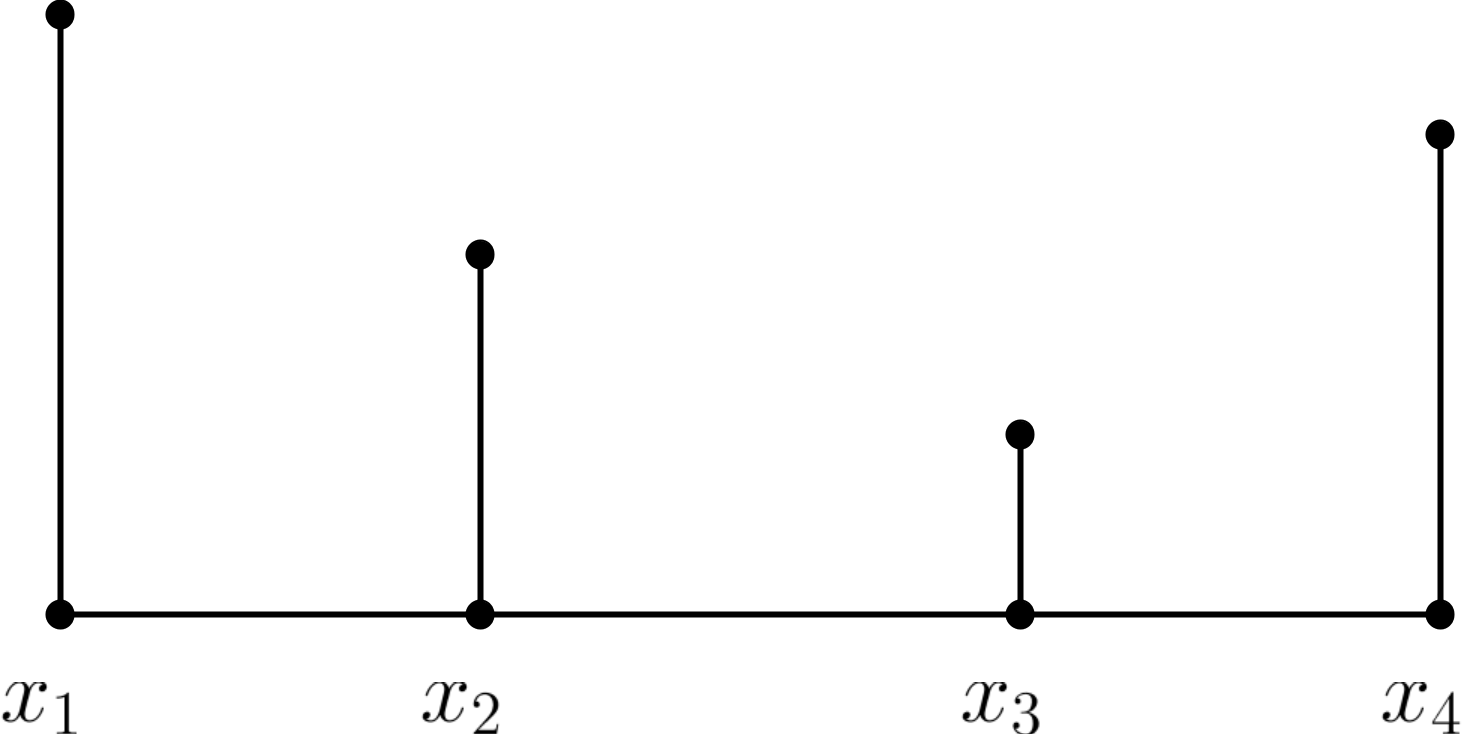
\includegraphics[width=8cm]{../aurea/aurea_fx.png}   
		\caption{Divisão áurea do segmento de reta}
		\label{fig:aurea_fx}
	\end{center}
\end{figure}

A figura \ref{fig:aurea_fx} ilustra a execução do método. É definido um intervalo que vai de $ x_1 $ até $ x_4 $ e dentro desse intervalo são escolhidos mais dois pontos, $ x_2 $ e $ x_3 $, porém dessa vez com a regra de divisão áurea. Depois disso, são calculados os valores da função objetivo que se deseja minimizar para os quatro pontos.

Tendo os dois valores $ f(x_2) $ e $ f(x_3) $, é selecionado o maior deles e o intervalo adjacente à esse é retirado. No caso da figura \ref{fig:aurea_fx}, o ponto $ x_1 $ seria retirado. Para continuar o método, é necessário que mais um ponto seja adicionado, novamente com a regra da razão áurea. Agora que temos novamente 4 pontos, o método pode ser repetido até que uma tolerância escolhida tenha sido atingida, e assim é localizado o mínimo da função.

Com o algoritmo da divisão áurea construído, foram testadas quatro funções para efeitos de comparação:

\begin{itemize}
	\item $ f_1(x) = 3x^2 + 20x - 8 $
	\item $ f_2(x) = xsin(x)cos(x) $
	\item $ f_3(x) = 5x $
	\item $ f_4(x) = -e^{-\mid x \mid} $
\end{itemize}

\newpage

Os resultados para a função $ f_1(x) $ foram:

\begin{figure}[h]
	\begin{center}
		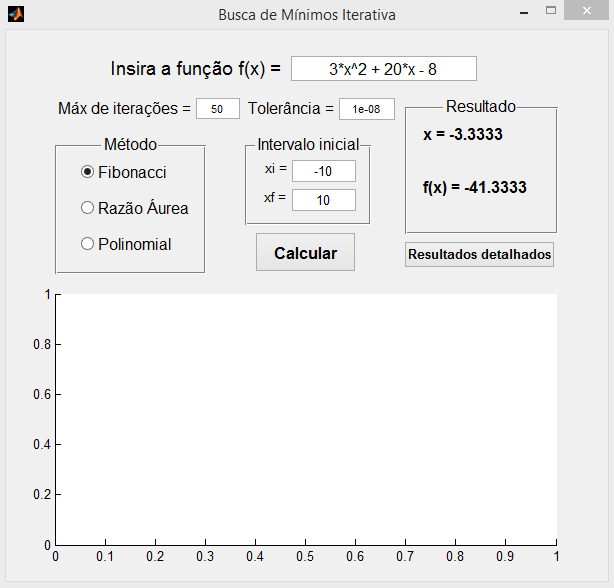
\includegraphics[width=14cm]{../aurea/f1_gui.png}   
		\caption{Janela de inicialização de $ f_1(x) $}
		\label{fig:f1_gui}
	\end{center}
\end{figure}

\begin{figure}[h!]
	\begin{center}
		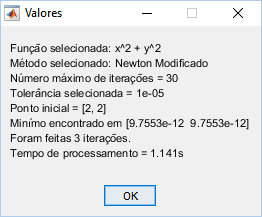
\includegraphics[width=6cm]{../aurea/f1_resultados.png}   
		\caption{Resultados detalhados de $ f_1(x) $}
		\label{fig:f1_resultados}
	\end{center}
\end{figure}

Os resultados para a função $ f_2(x) $ foram:

\begin{figure}[h]
	\begin{center}
		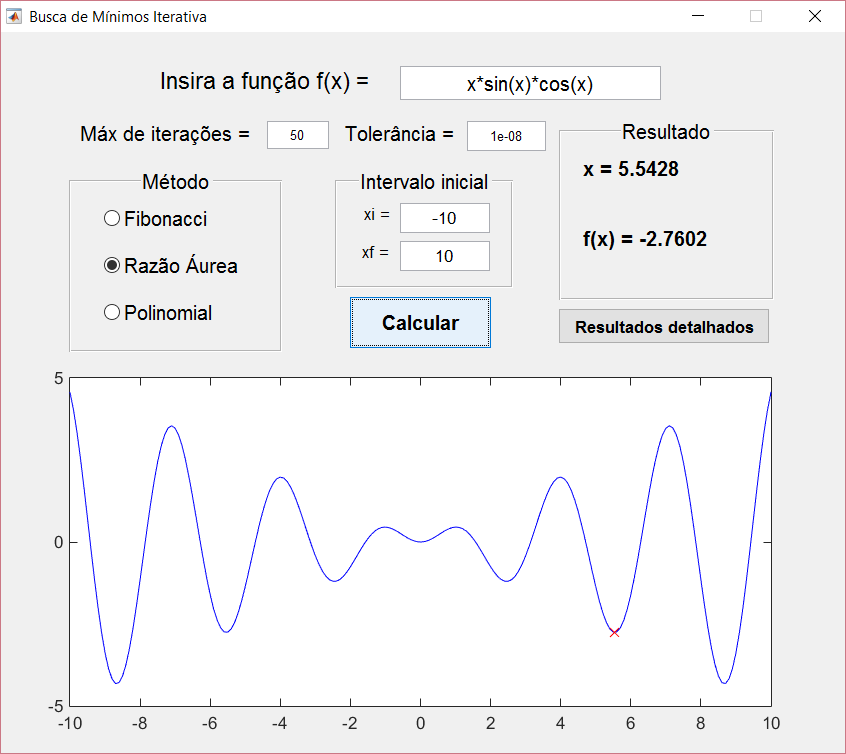
\includegraphics[width=14cm]{../aurea/f2_gui.png}   
		\caption{Janela de inicialização de $ f_2(x) $}
		\label{fig:f2_gui}
	\end{center}
\end{figure}

\begin{figure}[h!]
	\begin{center}
		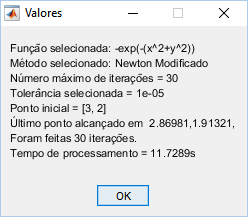
\includegraphics[width=6cm]{../aurea/f2_resultados.png}   
		\caption{Resultados detalhados de $ f_2(x) $}
		\label{fig:f2_resultados}
	\end{center}
\end{figure}

Os resultados para a função $ f_3(x) $ foram:

\begin{figure}[h]
	\begin{center}
		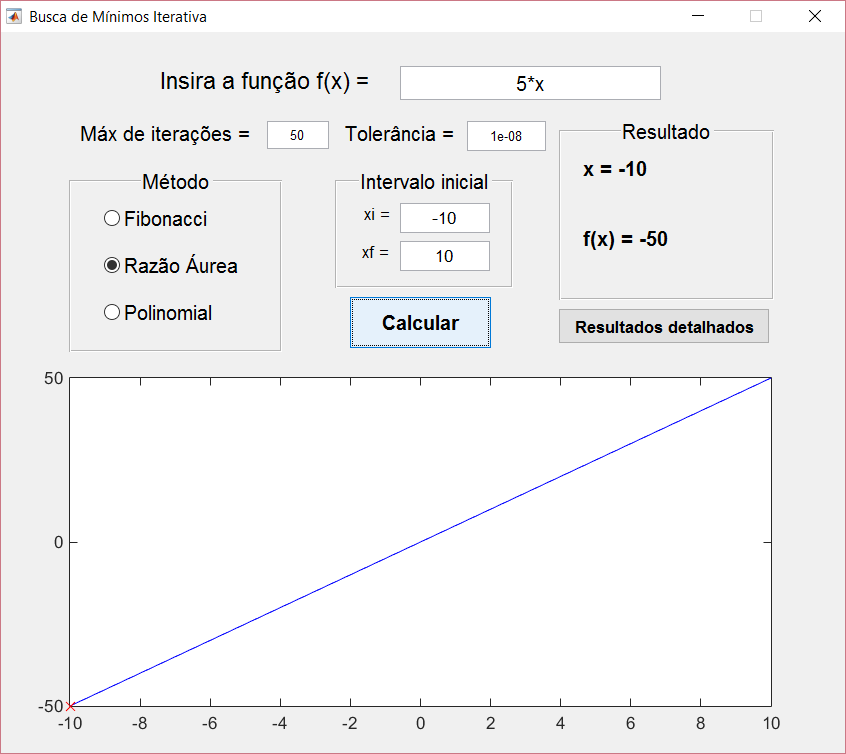
\includegraphics[width=14cm]{../aurea/f3_gui.png}   
		\caption{Janela de inicialização de $ f_3(x) $}
		\label{fig:f3_gui}
	\end{center}
\end{figure}

\begin{figure}[h!]
	\begin{center}
		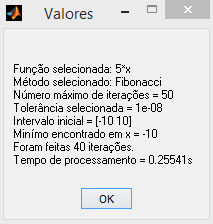
\includegraphics[width=6cm]{../aurea/f3_resultados.png}   
		\caption{Resultados detalhados de $ f_3(x) $}
		\label{fig:f3_resultados}
	\end{center}
\end{figure}

Os resultados para a função $ f_4(x) $ foram:

\begin{figure}[h]
	\begin{center}
		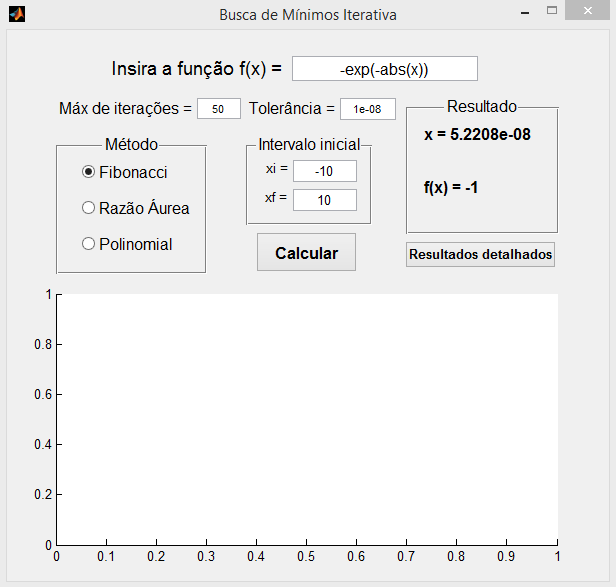
\includegraphics[width=14cm]{../aurea/f4_gui.png}   
		\caption{Janela de inicialização de $ f_4(x) $}
		\label{fig:f4_gui}
	\end{center}
\end{figure}

\begin{figure}[h!]
	\begin{center}
		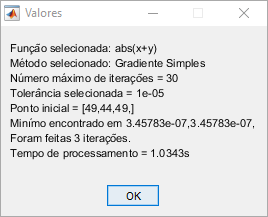
\includegraphics[width=6cm]{../aurea/f4_resultados.png}   
		\caption{Resultados detalhados de $ f_4(x) $}
		\label{fig:f4_resultados}
	\end{center}
\end{figure}
